\section{introduction}
% 1000-1500 words

%Coastal zones

The coastal ocean — the marine area extending from the coastline to the continental slope, encompassing the continental shelf — constitutes one of the most dynamic and complex regions of the ocean. These areas are characterized by highly variable forcing mechanisms, intricate topographies, and coastline geometries. They are forced by a wide range of physical and biogeochemical processes which occur across diverse spatial and temporal scales. They are among the most productive and economically significant areas of the world’s oceans, benefiting from terrestrial inputs via river discharges and nutrient renewal driven by upwelling processes.
Due to this richness, coastal areas concentrate a great proportion of human maritime activities, from fisheries and offshore aquaculture to renewable energy exploitation. Moreover, the coastal ocean acts as an interface between deep-ocean processes and coastal environment, modulating how large-scale phenomena — such as climate-driven changes or extreme weather events — impact coastal populations. It also regulates, for example, how anthropogenic influences originating on land are redistributed and affect marine ecosystems.

%need for forecasting
Recent events and ongoing changes in the coastal environment underscore the importance of understanding and predicting the behavior of these dynamic systems. The complex interplay between physical, chemical, and biological processes in the coastal ocean can rapidly amplify or modulate the impacts of extreme events such as storms, flooding, or pollution incidents. Furthermore, the coastal ocean serves as a key interface where large-scale oceanic and atmospheric changes manifest their consequences for coastal ecosystems. Accurately forecasting the state of the coastal ocean is therefore essential not only for safeguarding environmental and economic interests, but also for enhancing resilience to climate variability, natural hazards, and human-induced pressures. Achieving this, however, remains a major scientific and technological challenge, given the high variability, rapid dynamics, and observational constraints inherent to these regions.

%Models and data assimilation
Ocean models have become essential tools for predicting the ocean state and underpin a wide range of societal applications, from climate forecasting to pollution monitoring and resource management. However, these models are inherently imperfect representations of complex reality. Data assimilation techniques — where observational data are integrated into models — play a critical role in correcting or adjust model errors and improving their forecasting capabilities. Yet, the success of data assimilation heavily depends on the availability, quality, and relevance of observations.

%need for observations
Observations of the ocean are obtained through multiple sources. Satellite remote sensing offers extensive spatial coverage but is limited to surface viewing with usually low spatial resolution and often compromised by atmospheric conditions. In situ observations, whether from ships, moorings, or drifting platforms, provide higher accuracy but suffer from limited spatial and temporal coverage, high operational costs, and logistical constraints — particularly high in coastal regions and their phenomena. Recent technological advances have enabled the use of autonomous underwater vehicles (AUVs) and other robotic platforms, offering flexible, mobile, and increasingly autonomous means of sampling ocean properties with high spatiotemporal resolution and low logistic footprint.

%robotics applications
However, even with these new tools, efficiently gathering the \textit{right} data remains a complex challenge. AUVs are constrained by endurance, communication bandwidth, and operational risks. Meanwhile, the ocean itself remains highly dynamic and unpredictable, with key processes often evolving faster than traditional sampling strategies can capture. This opens the door to adaptive sampling strategies, where observation efforts are guided by model outputs and uncertainty estimates to maximize the informativeness of collected data. Adaptive sampling represents a fundamental shift: instead of executing pre-planned missions, autonomous vehicles dynamically prioritize areas for observation based on predicted model uncertainties in comparison with prior data assimilation process with availabe obervations. Model forecasts identify where uncertainty is highest or where new observations are expected to have the greatest impact in reducing forecast errors. Vehicles are then tasked to sample these areas, and their data are assimilated back into the models, generating improved forecasts for subsequent adaptive planning.

%data-cycle
This closes a critical feedback loop between models and observations:
\begin{itemize}
    \item Model prediction generates a forecast and associated uncertainty field.
    \item Adaptive sampling targets areas/routes of maximum predicted uncertainty.
    \item Data assimilation incorporates collected data into the model.
    \item New model prediction benefits from the improved data, closing the loop.
\end{itemize}

\begin{figure}
    \centering
    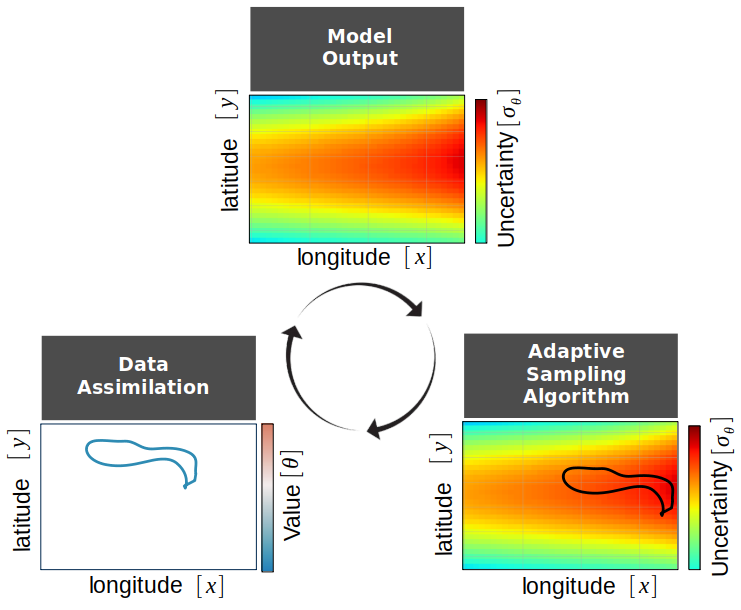
\includegraphics[width=.7\linewidth]{fig/data_cycle.png}
    \caption{Enter Caption}
    \label{fig:enter-label}
\end{figure}

The \textit{data cycle} approach promises to significantly enhance the skill of ocean forecasts, especially in the complex coastal environment where processes occur over a wide range of scales and where human and environmental stakes are high. It also has the potential to improve operational efficiency by optimizing the deployment of costly and resource-constrained observational assets.

% real-world gap
Yet, implementing such a system in the real world presents substantial challenges. It demands high-resolution numerical models capable of rapidly generating uncertainty projections, robust algorithms for path planning under vehicle and environmental constraints, reliable communication links for mission updates, and assimilation frameworks able to integrate heterogeneous, real-time data streams. Furthermore, the logistical risks and communication limitations inherent to marine operations — low bandwidth, intermittent connections, unpredictable weather conditions — impose additional constraints on the practical execution of adaptive sampling missions.

%impact
In this study, we address these challenges by implementing and evaluating a complete data cycle — from model prediction, to uncertainty projection, to adaptive sampling and data assimilation — in a real-world coastal ocean environment. The work was conducted within the framework of  \proj (\textbf{F}ield expe\textbf{R}iments for mod\textbf{E}ling,
a\textbf{S}similatio\textbf{N} and adaptiv\textbf{E}
samp\textbf{L}ing), a project specifically designed to explore and test model-driven exploration strategies. \proj provided the experimental setting and operational assets to demonstrate how model-based uncertainty fields can drive adaptive sampling missions aimed at improving ocean model predictive skills. This paper focuses on the underlying problem: how to effectively close the loop between model predictions, observational targeting, and data assimilation to enhance ocean forecasts in highly dynamic coastal environments. The experimental results obtained within \proj serve to illustrate and validate the proposed approach, highlighting the practical benefits and challenges of real-world adaptive ocean exploration.


% \textit{\textbf{-	Set the context and background of your study.}}
% \begin{itemize}
% \item Fresnel proposal context
% \item Data cycle idea
% \item Model predictions and uncertainties -$>$ Improve quality of Data gathering -$>$ data assimilation into models -$>$ better model predictions
% \item Point out the logistics difficulties of doing this in the sea (low bandwidth comms, risks, computing time, etc)
% \end{itemize}

% \textit{-	\textbf{Clearly state the objective and significance of your research.}}
% \begin{itemize}
% \item real-world experiment to close the data loop between better efficiency to get data to improve the Improved Ocean Model Predictions\
% \end{itemize}
% \begin{itemize}
%     \item present a figure showing that idea of loop/cycle
% \end{itemize}
